\documentclass[11pt]{article}
\usepackage[margin=1in]{geometry}
\usepackage{graphicx}
\usepackage{booktabs}
\usepackage{amsmath}
\usepackage{amssymb}
\usepackage{xcolor}
\usepackage[hidelinks]{hyperref}
\usepackage{caption}
\captionsetup{font=small}

\newcommand{\reconear}{\texttt{reco\_near}}
\newcommand{\recofar}{\texttt{reco\_far}}

\title{\vspace{-2.5em}Characterisation of the \recofar\ events for detector~3\\
\large (June cosmic bench --- \texttt{g\_det3\_wknd})}
\author{MX17 cosmic-bench QA}
\date{\today}

\begin{document}
\maketitle
\vspace{-1.5em}

\section{Setup and definitions}
For every clean M3 reference muon crossing the det3 active area we ask where the
detector's reconstructed $X{+}Y$ point lands relative to the M3 ray projection:
%
\begin{itemize}\setlength\itemsep{0.1em}
  \item \reconear: valid reco point, $|r|\le 5$~mm (this is the efficiency);
  \item \recofar: valid reco point, but $|r|>5$~mm;
  \item \texttt{spark}: event fires $>50$ strips (a full-detector discharge), pulled
        out \emph{before} the reco/hit split so it does not contaminate the tail;
  \item \texttt{hit\_no\_reco} / \texttt{no\_hit}: fired but no valid point / silent.
\end{itemize}
%
Run \texttt{mx17\_det3\_p2\_det1\_overnight\_6-27-26 / long\_run\_p2}, the headline det3
page. Numbers below reproduce the June overview PDF exactly.

\begin{table}[h]\centering\small
\begin{tabular}{lrr}
\toprule
category & $N$ & \% of active-area crossings\\
\midrule
\reconear\ ($\le 5$~mm) & 41\,743 & 78.8\,\%\\
\recofar\ ($>5$~mm)     & \textbf{7\,271}  & \textbf{13.7\,\%}\\
\texttt{spark} ($>50$ strips) & 2\,600 & 4.9\,\%\\
\texttt{hit\_no\_reco}  & 85    & 0.2\,\%\\
\texttt{no\_hit} (silent) & 1\,296 & 2.4\,\%\\
\midrule
total crossings & 52\,995 & 100\,\%\\
\bottomrule
\end{tabular}
\caption{det3 breakdown (sparks already removed). The 13.7\,\% \recofar\ tail is the
subject of this note.}
\end{table}

\section{Result in one paragraph}
The \recofar\ tail is \emph{not} uniform and \emph{not} a tracking artefact. It is
two overlapping populations: (i) a \textbf{near-miss} shoulder just outside the 5~mm cut
(41\,\% of \recofar\ sit at $5$--$10$~mm), which is the ordinary resolution/angle tail;
and (ii) a genuine \textbf{mis-reconstruction} tail ($38\,\%$ beyond $20$~mm, $23\,\%$
beyond $50$~mm) that is driven by \textbf{elevated-multiplicity ``sub-veto'' discharge
activity}, spatially \textbf{concentrated on one side of the detector (low $X$ / left
edge)}. The multi-ray / ray-mismatch hypothesis is cleanly ruled out ($0\,\%$ of
\recofar\ events have more than one M3 ray).

\section{Where they are: a localised low-$X$ (left-edge) region}
Figure~\ref{fig:where} is the key plot. Both the muon crossings that go \recofar\
(panel a) and --- more sharply --- the detector positions where the bad reco point
\emph{lands} (panel c) pile up on the low-$X$ (left) side of the chamber. The
\recofar\ \emph{rate} map (panel b) is $\sim 10\,\%$ in the bulk but rises to
$25$--$70\,\%$ along the left edge and around the periphery (median $14\,\%$,
$90^{\text{th}}$ pct $25\,\%$). A wrong reco point preferentially reconstructs into
the low-$X$ band regardless of where the muon actually crossed --- the signature of a
localised noisy / spark-prone detector region generating displaced clusters, not a
global reconstruction bias.

\begin{figure}[h]\centering
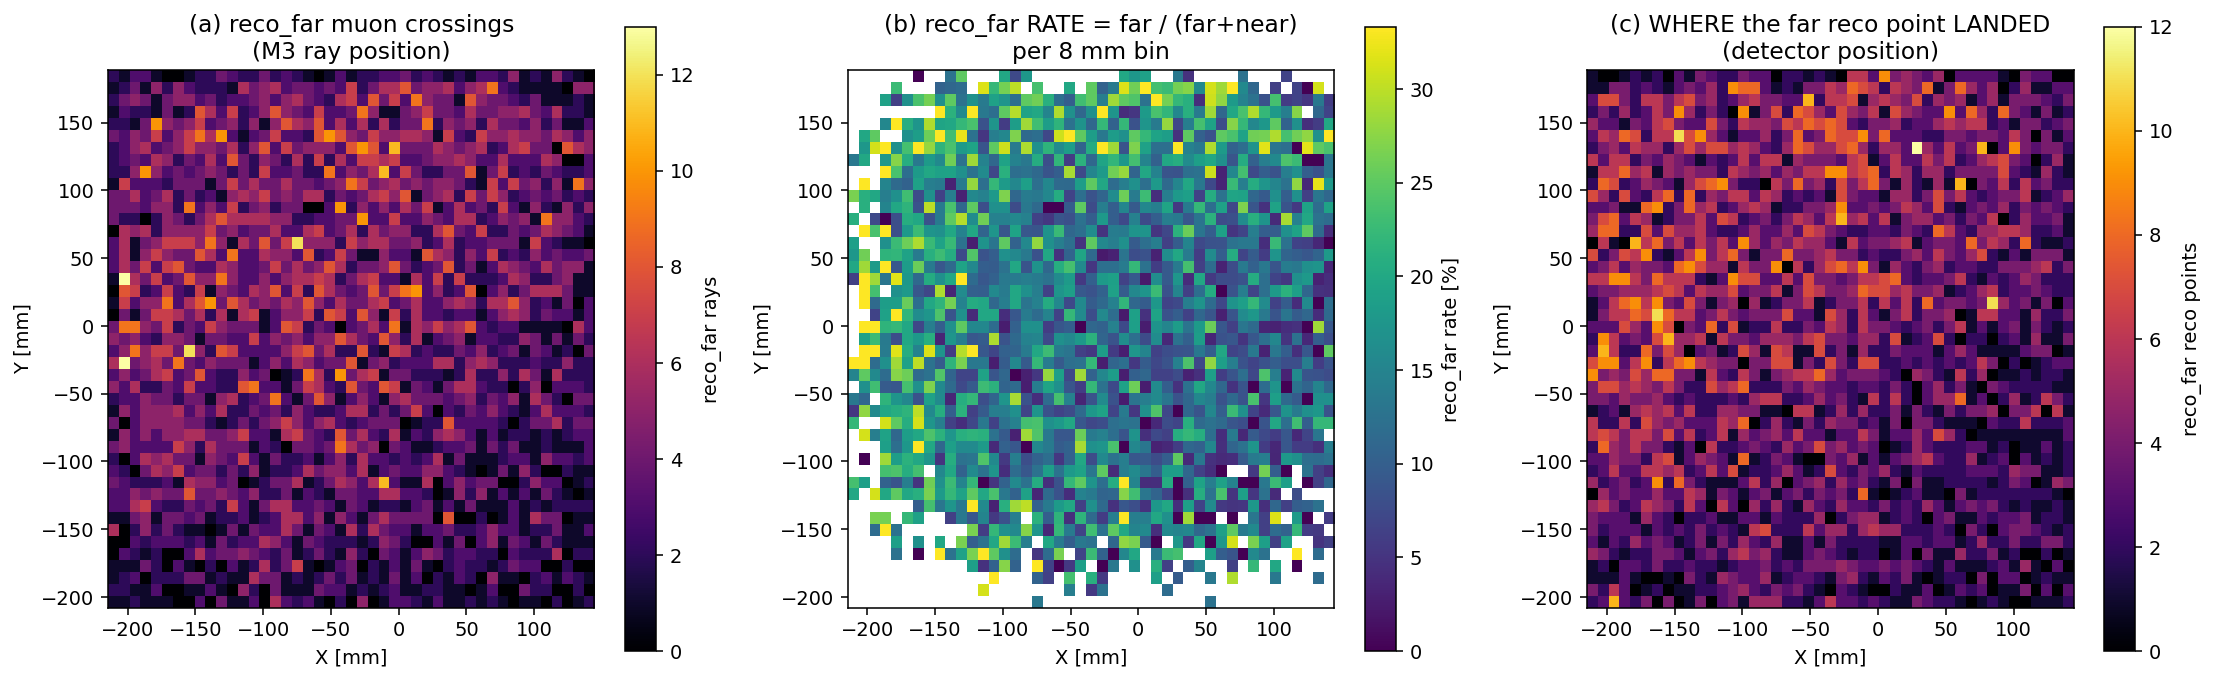
\includegraphics[width=\textwidth]{fig_where.png}
\caption{\textbf{Spatial distribution.} (a) M3 crossing positions of \recofar\ muons;
(b) \recofar\ rate $=$ far$/$(far$+$near) per $8$~mm bin (bins with $\ge15$ tracks);
(c) detector positions where the far reco point landed. The low-$X$ / left-edge
region dominates both the rate and the landing points.}
\label{fig:where}
\end{figure}

\section{What kind of events: elevated multiplicity, sub-veto discharges}
\recofar\ events fire \emph{more} strips than \reconear\ ones (median $20$ vs $16$;
$90^{\text{th}}$ pct $39$ vs $23$), with a population piling up against the $50$-strip
spark veto (Fig.~\ref{fig:what}a). These are ``half-sparks'': the same discharge
phenomenon as the vetoed sparks, but sitting in the $20$--$50$ strip shoulder just below
the cut, where they survive into the reco categories and throw spurious displaced
clusters. The effect strengthens with $|r|$: the genuinely-wrong tail ($>20$~mm) has
median multiplicity $26$ versus $18$ for the $5$--$10$~mm near-misses. A long-duration
cluster tail corroborates this --- the mean $X$ cluster duration is $3888$~ns for
\recofar\ versus $581$~ns for \reconear\ (Fig.~\ref{fig:what}c), i.e.\ a subset of
multi-pulse / afterpulsing clusters. Fitted cluster sizes are only mildly larger
(median $9$ vs $8$ strips, panel b).

\begin{figure}[h]\centering
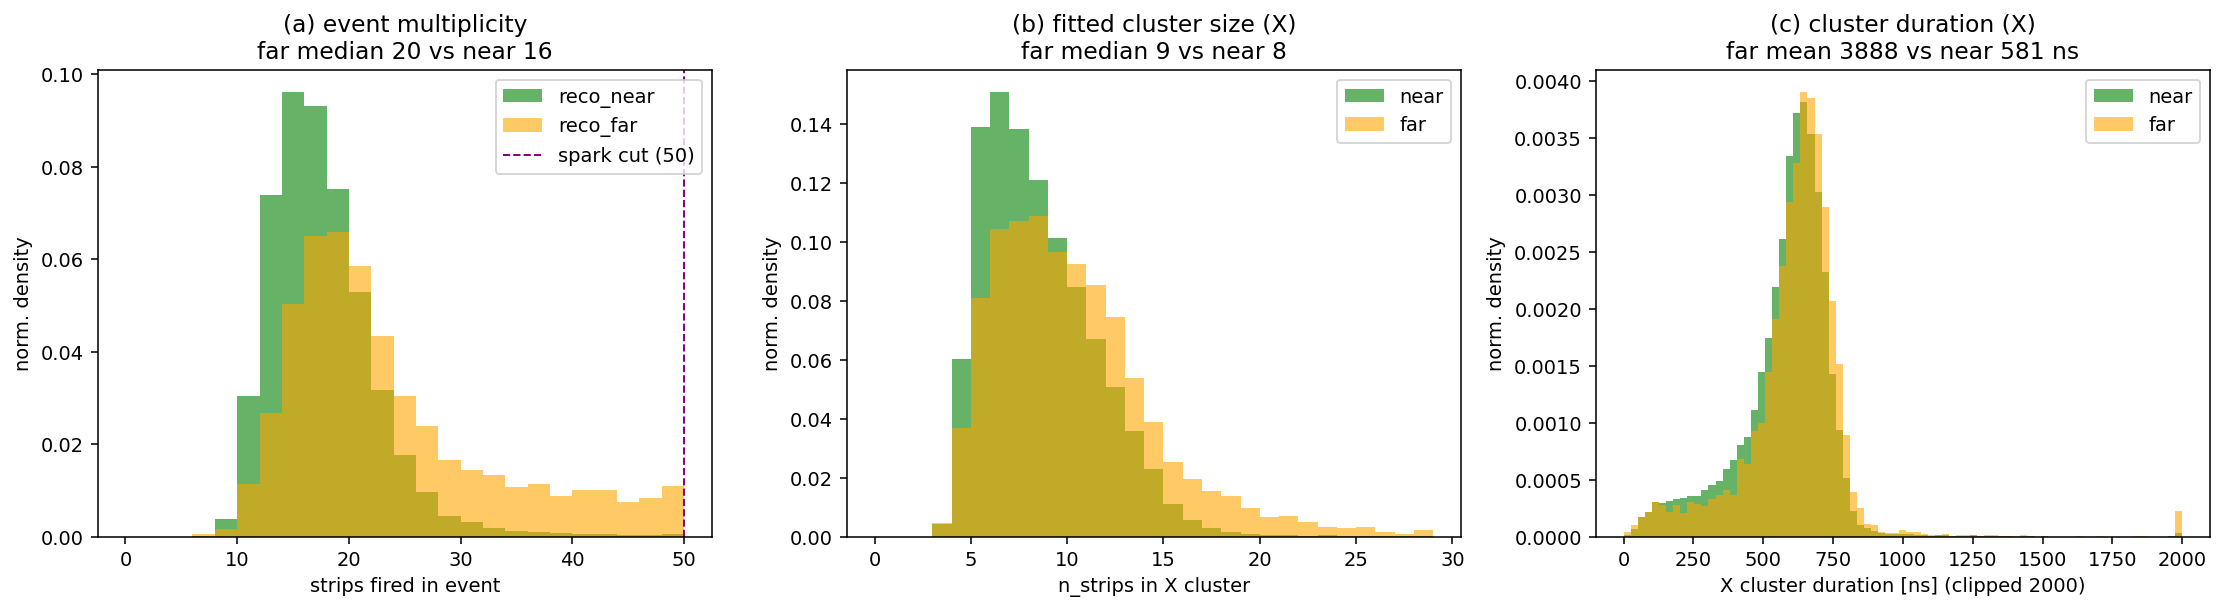
\includegraphics[width=\textwidth]{fig_what.png}
\caption{\textbf{Event character (far vs near, area-normalised).} (a) strips fired per
event --- \recofar\ extends toward the $50$-strip spark cut; (b) fitted $X$-cluster
size; (c) $X$-cluster duration --- \recofar\ has a heavy long-duration (multi-pulse)
tail (note the pile-up at the $2000$~ns clip).}
\label{fig:what}
\end{figure}

\section{Which plane fails, and the multi-ray cross-check}
No single readout plane is responsible: of the \recofar\ events, $35.6\,\%$ have only
the $X$ plane displaced, $23.5\,\%$ only $Y$, and $40.9\,\%$ have \emph{both} planes
wrong (threshold $5/\sqrt2\approx3.5$~mm). The per-plane displacement map
(Fig.~\ref{fig:planes}b) shows the corresponding ``cross-plus-cloud'': bright axis arms
(one plane correct, one wrong = the near-miss shoulder) sitting on a diffuse both-wrong
cloud (the genuine tail). The radial residual (Fig.~\ref{fig:planes}a) falls smoothly
from the $5$~mm cut and flattens into a wide $>50$~mm plateau extending across the whole
chamber --- consistent with clusters landing at essentially random wrong positions.

Finally, the ray-mismatch hypothesis is excluded: \textbf{$0.00\,\%$} of \recofar\
(and of \reconear) events carry more than one accepted M3 ray after the $\chi^2<20$
cut, so a ``detector saw the other track'' explanation does not apply to this run.

\begin{figure}[h]\centering
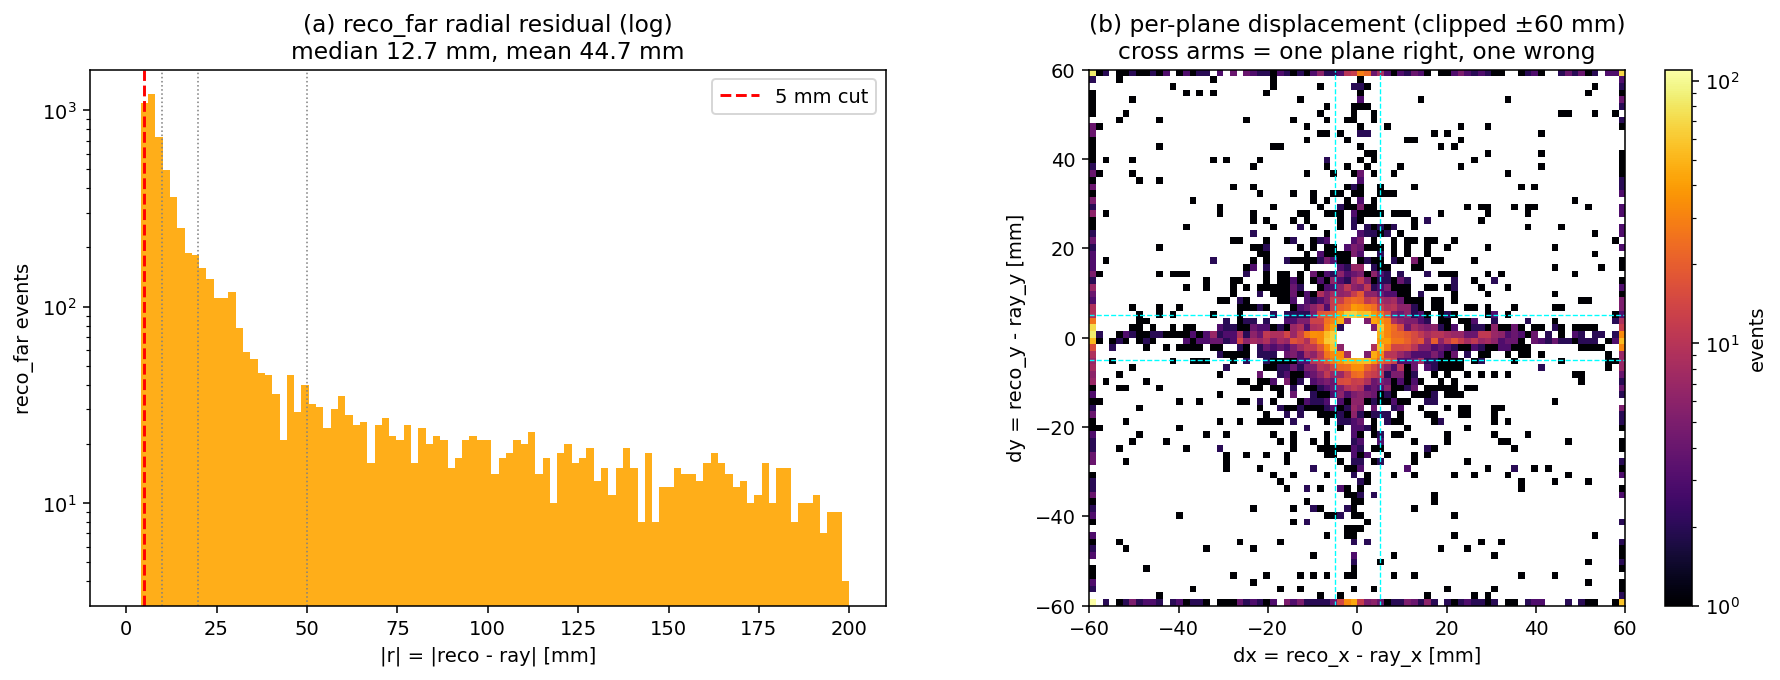
\includegraphics[width=0.92\textwidth]{fig_residual_planes.png}
\caption{\textbf{Residual structure.} (a) \recofar\ radial residual (log $y$): smooth
fall-off plus a flat far plateau. (b) per-plane displacement $(\mathrm{d}x,\mathrm{d}y)$,
clipped $\pm60$~mm; cyan lines mark $\pm5$~mm. The cross arms are one-plane-wrong events;
the diffuse cloud is both-planes-wrong.}
\label{fig:planes}
\end{figure}

\section{Interpretation and takeaways}
\begin{itemize}\setlength\itemsep{0.15em}
  \item About $\mathbf{40\,\%}$ of the \recofar\ tail is a benign $5$--$10$~mm near-miss
        shoulder --- the resolution/angle tail spilling just past the $5$~mm cut. Widening
        the cut to $\sim7$~mm, or the existing core-$\sigma$ metric, already accounts for it.
  \item The remaining, genuinely-wrong tail ($\gtrsim20$~mm, $\sim38\,\%$) is a
        \textbf{detector/HV effect}: sub-veto discharges ($20$--$50$ strips, long
        multi-pulse clusters) concentrated in the \textbf{low-$X$ / left-edge} region,
        producing displaced competing clusters that the micro-TPC fit sometimes selects.
  \item It is \emph{not} a tracking or ray-matching problem (multi-ray $=0\,\%$) and
        \emph{not} a single-plane readout fault (both planes contribute).
  \item \textbf{Suggested follow-ups:} (1) tighten the discharge veto toward
        $\sim30$--$40$ strips (or add a cluster-duration / multi-pulse veto) and re-measure
        --- most of the genuine tail should move into a \texttt{spark}-like category;
        (2) inspect the low-$X$ edge strips for HV/sparking or common-mode noise; (3) at
        the waveform level, confirm the $>20$~mm events show discharge/afterpulse
        signatures rather than clean muon clusters.
\end{itemize}

\vspace{0.5em}
\footnotesize\noindent\textit{Reproduce:} \texttt{extract\_recofar.py} (categorise +
join to \texttt{EventResult}) then \texttt{make\_plots.py}; numbers in
\texttt{recofar\_meta.json}. Categorisation matches \texttt{09\_efficiency\_breakdown.py}
(same alignment, active box, and $50$-strip spark cut).

\end{document}
